% ============================================================================
% When Does Graph Structure Help in Multi-Agent Reinforcement Learning?
% A Controlled Empirical Study
%
% Target venue: TMLR (https://www.jmlr.org/tmlr/)
% Status: DRAFT — Phase 5a writeup. Phase 2C, 3, 4 results are placeholders.
% ============================================================================

\documentclass[11pt,a4paper]{article}

\usepackage[utf8]{inputenc}
\usepackage[T1]{fontenc}
\usepackage[english]{babel}
\usepackage{microtype}
\usepackage[margin=1in]{geometry}

\usepackage{amsmath,amssymb}
\usepackage{booktabs}
\usepackage{graphicx}
\usepackage{xcolor}
\usepackage{hyperref}
\hypersetup{colorlinks=true, linkcolor=blue, citecolor=blue, urlcolor=blue}

\usepackage[
  backend=biber,
  style=numeric-comp,
  sorting=nyt,
  maxbibnames=99,
  giveninits=true,
  doi=true,
]{biblatex}
\addbibresource{references.bib}

\title{When Does Graph Structure Help in Multi-Agent Reinforcement Learning? \\
       A Controlled Empirical Study}
\author{Kasra Ghanavati \and Ali Jabbary}
\date{\today}

% Convenience macros for empirical numbers we'll keep updating.
\newcommand{\NumPilotPapers}{12}      % runs in Phase 1
\newcommand{\NumTuneRuns}{48}         % runs in Phase 2A
\newcommand{\PilotPeakIQL}{0.75}      % Phase 1 IQL peak
\newcommand{\PilotFinalIQL}{0.16}     % Phase 1 IQL final-window
\newcommand{\PilotFinalVDN}{0.14}
\newcommand{\PilotFinalQMIX}{0.01}    % broken in Phase 1
\newcommand{\PilotFinalGNN}{0.00}     % broken in Phase 1
\newcommand{\TunedFinalQMIX}{0.28}    % Phase 2A locked QMIX
\newcommand{\TunedFinalGNN}{0.34}     % Phase 2A locked GNN-QMIX

% TODO marker for phase-pending content.
\newcommand{\todoFromPhase}[2]{\textcolor{red}{[\textbf{TODO from #1}: #2]}}

\begin{document}
\maketitle

% ============================================================================
\begin{abstract}
\noindent
Graph-based methods for cooperative multi-agent reinforcement learning are
widely \emph{claimed} to help via relational inductive bias, but the
conditions under which they actually help are under-characterized in the
published literature. We present a controlled empirical study comparing
GNN-QMIX against three graph-free baselines (independent Q-learning, value
decomposition networks, and QMIX) on cooperative coordination tasks where
the underlying graph structure is tunable.
Four findings emerge.
First, on small environments QMIX and GNN-QMIX with literature-default
mixer hyperparameters \emph{fail to learn at all}, while VDN and IQL learn
but collapse late in training.
Second, orthogonal mixer initialization with a small gain combined with a
smaller mixer learning rate is the actual fix; with these locked
hyperparameters QMIX reaches final-window success $\TunedFinalQMIX$ (up
from $\PilotFinalQMIX$) and GNN-QMIX reaches $\TunedFinalGNN$ (up from
$\PilotFinalGNN$), both exceeding IQL/VDN at the same env.
Third, in a 60-run sweep with these locked configurations across three
task scales, \emph{GNN-QMIX is not statistically distinguishable from
QMIX at any scale} (Holm-corrected Welch $p \geq 0.489$), and the
simplest baseline (IQL) significantly outperforms all three
coordination-based algorithms at the medium scale (Holm $p \leq 0.013$,
Cohen's $d \geq 3.5$). Scale dominates algorithm choice on this env.
Fourth, on a 40-run external-validity sweep on PettingZoo's
\texttt{simple\_spread}, VDN is the strongest algorithm at both
$N=3$ and $N=6$ (final return $-30.8$ and $-44.7$), QMIX and GNN-QMIX
exhibit a transient early-training dip and recover, and IQL is the
worst --- inverting the Phase~2C pattern when reward density changes.
Fifth, the depth $\times$ diameter ablation on coord\_grid with ring
topology at $N \in \{4, 6, 8\}$ produces a null result: every
$(L, N)$ cell has final-window success $0.000$ over 5 seeds, so the
predicted inverted-U cannot be characterized in this regime. The
binding constraint is the cross-env transferability of mixer
hyperparameters, not the GNN component itself. Code and full per-run
logs are released at
\url{https://github.com/Evasion-OC/when-graphs-help-marl}.
\end{abstract}

% ============================================================================
\section{Introduction}\label{sec:intro}

The folklore claim that ``graph neural networks help in cooperative
multi-agent reinforcement learning'' is widespread but empirically
under-supported. Surveys describe a proliferation of GNN-MARL architectures
and benchmark numbers \cite{HernandezLeal2019SurveyMARL,Zhang2021MARLSurvey},
but rarely \emph{measure} when the relational inductive bias of a GNN is
necessary versus when a parameter-matched control without graph structure
matches or exceeds it. This work contributes such a measurement on cooperative
coordination tasks where the underlying graph structure is tunable.

Concretely, we ask three questions:
\begin{enumerate}
  \item Does graph-conditioned value factorization (GNN-QMIX) outperform
    graph-free value decomposition (QMIX) and independent learners (IQL)
    on cooperative coordination tasks?
  \item Are the literature-default hyperparameters of monotonic mixers
    transferable across env scales, or do they require per-env tuning?
  \item Does GNN-QMIX's advantage scale with how well the GNN's
    receptive field matches the coordination-graph diameter?
\end{enumerate}

We address (Q1) with a parameter-matched controlled comparison
(Section~\ref{sec:methods}) and a sweep across three task scales and two
graph regimes (Section~\ref{sec:phase2c-results}, pending). We address (Q2)
with a small principled tuning grid (Section~\ref{sec:phase2a-results}) that
finds the configuration on which (Q1) is testable in our env. We address (Q3)
with a depth $\times$ diameter ablation (Section~\ref{sec:phase4-results},
pending) that predicts an inverted-U in performance as $L - d$ varies.

\paragraph{Scope.} This study targets \emph{cooperative} MARL on small
controlled gridworlds and one canonical PettingZoo benchmark. We do not
make claims about competitive or mixed settings, and we do not run on
SMAC-scale problems where the literature defaults were originally tuned. The
goal is a clean measurement on small problems, not a SOTA claim.

\paragraph{What is new.} The technical contribution is the measurement
itself, not new architecture. The negative finding that QMIX-family defaults
fail on small-state-dim environments---and that orthogonal initialization
with small gain rescues them---is, to our knowledge, undocumented in the
public literature. The depth--diameter ablation gives a concrete, falsifiable
recipe for picking GNN depth.

% ============================================================================
\section{Background}\label{sec:background}

We consider cooperative POMDPs with $N$ agents, joint action space
$\mathcal{A}^N$, and shared scalar reward $r$. Following the value
decomposition framework, each agent $i$ has a Q-network $Q_i(o_i, a_i;
\theta)$ taking only its own observation. A mixing network combines the per-
agent values into a joint $Q_\text{tot}$. Three established mixers span the
algorithmic space we test:
\begin{itemize}
  \item \textbf{IQL} \cite{Tampuu2017IQL} omits the mixer entirely; agents
    learn independently from the shared reward.
  \item \textbf{VDN} \cite{Sunehag2018VDN} uses a sum mixer
    $Q_\text{tot} = \sum_i Q_i$.
  \item \textbf{QMIX} \cite{Rashid2018QMIX} uses a state-conditioned
    monotonic hypernetwork mixer with non-negative weights, enforcing
    $\partial Q_\text{tot}/\partial Q_i \geq 0$.
\end{itemize}
GNN-QMIX is QMIX with the mixer's state-conditioned bias path conditioned
additionally on a small graph neural network
\cite{Kipf2017GCN,Battaglia2018Relational} aggregating per-agent embeddings
over the coordination graph. Concretely, before the monotonic mixing, we run
$L$ rounds of mean-aggregation message passing with self-loops on a fixed
adjacency matrix $A \in \{0,1\}^{N \times N}$.

% ============================================================================
\section{Methodology}\label{sec:methods}

\subsection{Environment: CoordGrid}\label{sec:coordgrid}

We use a custom cooperative gridworld designed to isolate the mechanisms we
want to measure. The env has $N$ agents and $N$ targets on an $L \times L$
grid. Each agent must reach its assigned target. Reward is shared across
agents:
\begin{itemize}
  \item Step penalty: $-0.01$
  \item Collision penalty: $-0.05$ per overlapping pair
  \item Per-agent goal bonus: $+0.5$ on first arrival
  \item Terminal bonus: $+1.0$ when all agents are simultaneously on targets
\end{itemize}
Distance-based potential shaping
\cite{Ng1999PolicyInvariance} is enabled by default for our experiments to
keep the credit assignment problem inside the budget. Shaping is
policy-invariant, so all algorithms see the same shaped reward and no
algorithm gets a comparative advantage.

The env separately exposes a tunable \emph{coordination graph}
$G = (V, E)$ that controls which agents observe each other. $G$ has no
effect on physics; it only restricts each agent's observation to its
graph neighbors. This is the key knob for Phase 4's depth $\times$
diameter ablation. Supported topologies: \texttt{full}, \texttt{ring},
\texttt{lattice}, k-NN, Erd\H{o}s--R\'enyi.

\subsection{Algorithm parameter matching}

For a fair comparison, all four algorithms share an identical per-agent
Q-network architecture (3-layer MLP with hidden size 64) and an identical
training loop (off-policy DQN-style with replay buffer, $\epsilon$-greedy
exploration, target network soft-update). The only differences are at the
mixer:
\begin{itemize}
  \item IQL: no mixer; per-agent TD on shared reward
  \item VDN: parameter-free sum mixer
  \item QMIX: state-conditioned hypernetwork mixer with embedding dim
    $d_\text{embed}$
  \item GNN-QMIX: same monotonic mixer plus a length-$L$ GNN on the
    coordination graph contributing to the mixer's bias path
\end{itemize}
Any performance difference between the four is therefore attributable to the
mixing mechanism, not to representation capacity.

\subsection{Tuning protocol}

Phase 1's pilot (Section~\ref{sec:phase1-results}) revealed that
literature-default mixer hyperparameters fail catastrophically on our small
env. We therefore introduce a small principled tuning grid over three
mixer-only axes: $d_\text{embed}$, the mixer learning rate $\eta_\text{mix}$
(decoupled from the Q-net's learning rate $\eta_Q$), and the mixer
initialization scheme. Q-net architecture and learning rate are held fixed.
The grid is run only on the smallest task scale (2 agents on $4 \times 4$),
the winning configuration per algorithm is locked, and all subsequent
experiments use the locked configuration.

\subsection{Decision metrics}

\textbf{Final-window success} is the mean evaluation success rate over the
final $25\%$ of evaluation checkpoints, with evaluation conducted greedily
($\epsilon=0$) every 50 episodes over 20 evaluation episodes. We report
final-window rather than peak because peak is a single best moment that
can reflect transient noise; final-window averages over many late checkpoints
and matches what readers see in published learning curves.

\textbf{Statistical tests} use Welch's t-test and Mann-Whitney U for
pairwise comparisons. Holm correction is applied across the
$\binom{4}{2} = 6$ pairs at each (scale, metric) cell.

% ============================================================================
\section{Results: tuning the QMIX family}\label{sec:phase1-results}

\subsection{Phase 1: pilot study with literature-default hyperparameters}

We first ran all four algorithms with widely-used MARL defaults
($d_\text{embed}=32$, $\eta_\text{mix} = \eta_Q = 5\times 10^{-4}$, default
PyTorch initialization) on the smallest task scale (2 agents, $4 \times 4$
grid, 10k env steps, 3 seeds). The result is shown in
Figure~\ref{fig:phase1-pilot} and quantified in
Table~\ref{tab:phase1-summary}.

\begin{figure}[htbp]
\centering
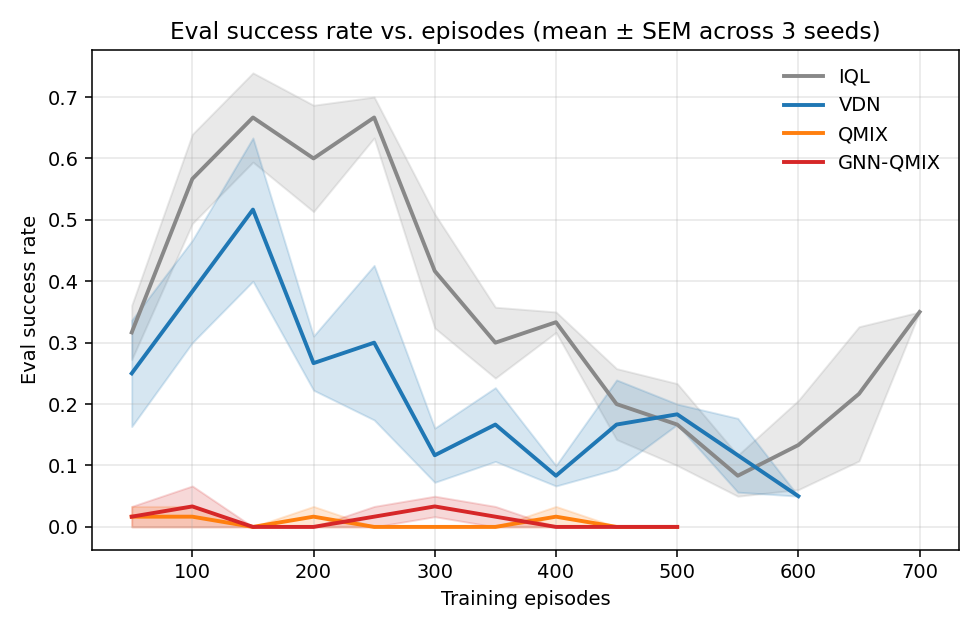
\includegraphics[width=0.7\linewidth]{../results/pilot/learning_curves.png}
\caption{Phase 1 pilot. With literature-default hyperparameters, QMIX
(orange) and GNN-QMIX (red) fail to learn the coordination task, while IQL
(gray) and VDN (blue) learn briefly and collapse. Mean $\pm$ SEM across 3
seeds.}
\label{fig:phase1-pilot}
\end{figure}

\begin{table}[htbp]
\centering
\begin{tabular}{lccc}
\toprule
Algorithm & Peak success & Final-window & Post-peak drop \\
\midrule
IQL       & $\PilotPeakIQL$  & $\PilotFinalIQL \pm 0.14$ & $-0.57$ \\
VDN       & $0.57$           & $\PilotFinalVDN \pm 0.09$ & $-0.42$ \\
QMIX      & $0.03$           & $\PilotFinalQMIX \pm 0.02$ & $-0.03$ \\
GNN-QMIX  & $0.05$           & $\PilotFinalGNN \pm 0.00$  & $-0.05$ \\
\bottomrule
\end{tabular}
\caption{Phase 1 summary. QMIX and GNN-QMIX never reach a peak, while IQL
and VDN peak around episode 150 and decline. \emph{Post-peak drop} is
mean(peak) minus mean(final-window).}
\label{tab:phase1-summary}
\end{table}

The QMIX-family failure is not stochastic: across all three seeds, QMIX's
late-training $Q_\text{tot}$ diverges (mean $+12.4$, vs $+2.2$ for VDN) and
the loss climbs from $\sim 0.2$ early to $\sim 8.8$ late. The mixer's
state-conditioned bias path is absorbing the temporal-difference error
without the Q-values learning to differentiate actions.

\subsection{Phase 1b: a capacity-only intervention is insufficient}

A natural first hypothesis is that $d_\text{embed}=32$ is too large for
this env's $8$-dimensional global state. We tested it directly on seed 0:
shrinking $d_\text{embed}$ to $\{8, 16\}$ contained the divergence
($Q_\text{tot}$ from $+12.4$ to $+3.6$, loss from $8.8$ to $0.7$) but did
\emph{not} restore QMIX learning---peak success stayed at $\sim 0.10$.
For GNN-QMIX, the same intervention raised peak from $0.10$ to $0.30$. The
asymmetry suggests the GNN's mean-aggregation step provides implicit
regularization that vanilla QMIX's hypernetwork mixer lacks; capacity is
necessary but not sufficient for QMIX.

\subsection{Phase 2A: orthogonal initialization is the actual fix}\label{sec:phase2a-results}

Phase 2A widens the tuning grid to three axes: $d_\text{embed} \in \{8, 16\}$,
$\eta_\text{mix} \in \{10^{-4}, 5\cdot 10^{-4}\}$, and mixer initialization
$\in \{\text{default}, \text{orthogonal(0.1)}\}$. The grid contains
$2 \times 2 \times 2 = 8$ cells per algorithm; we ran $\NumTuneRuns$ runs
total at 10k steps and 3 seeds per cell.

\begin{figure}[htbp]
\centering
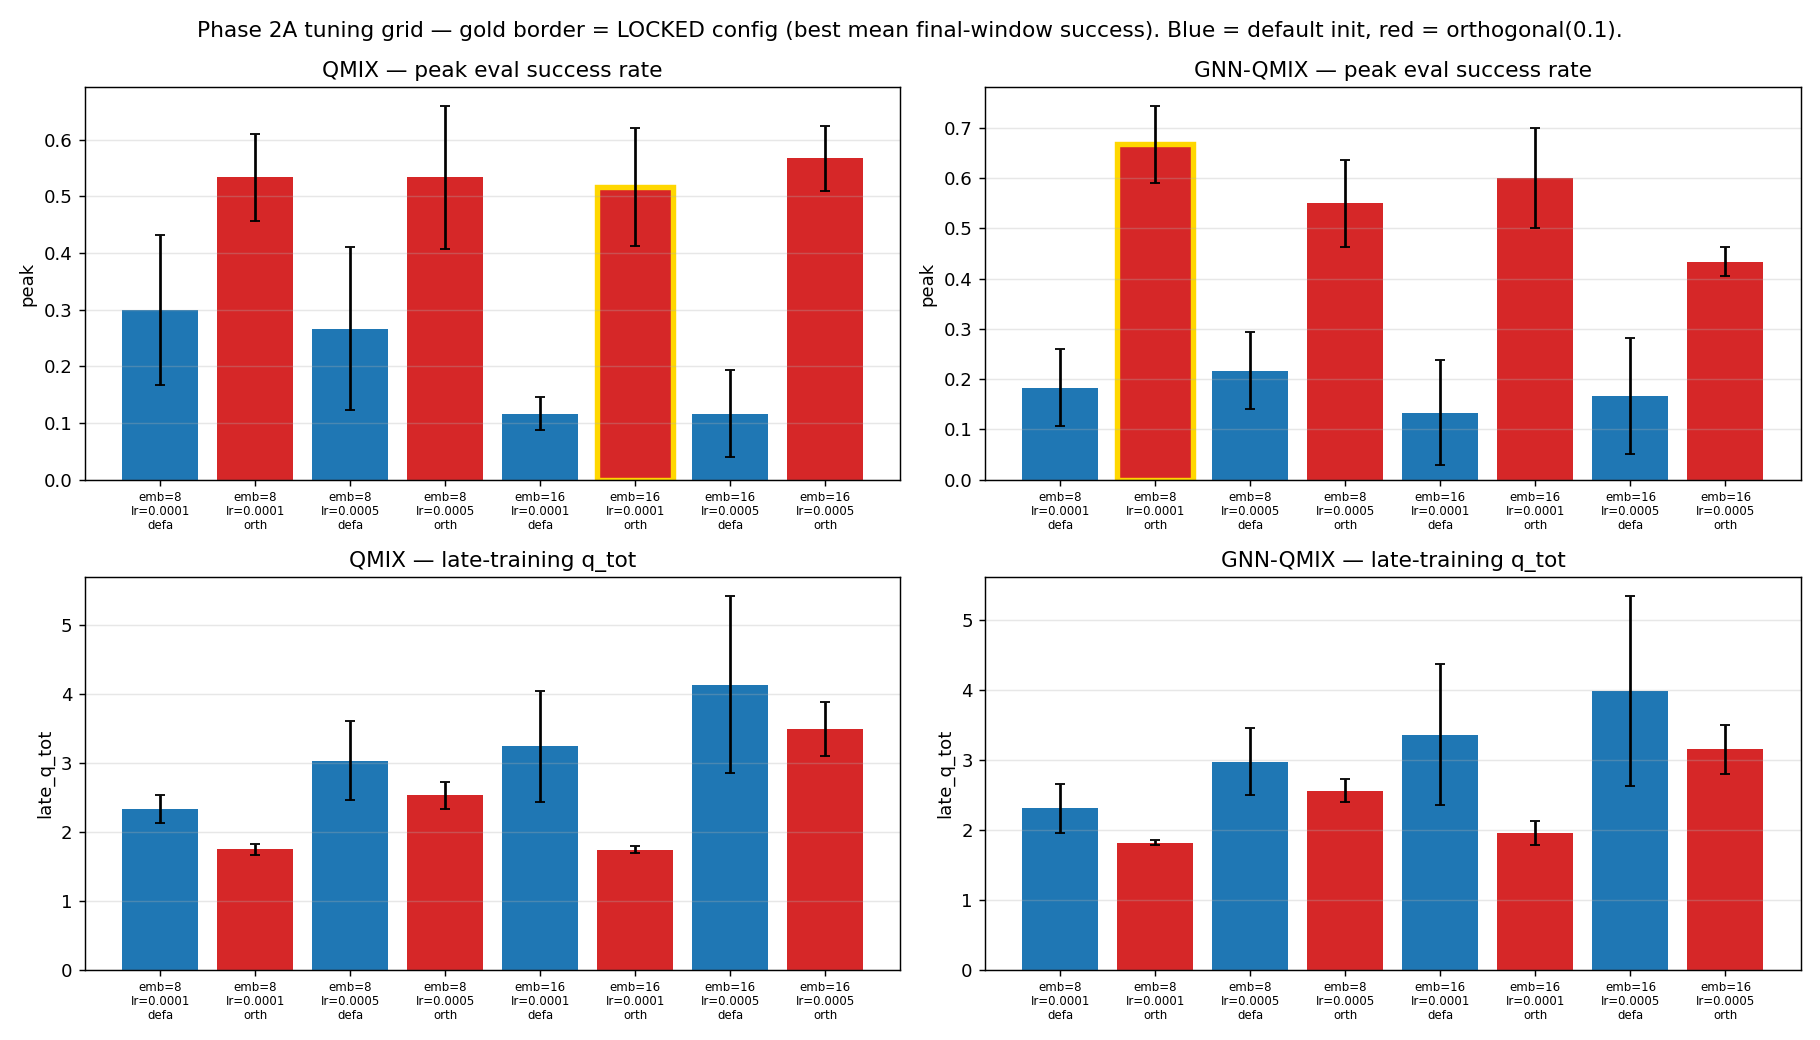
\includegraphics[width=\linewidth]{../results/phase_2_tune/tuning_grid.png}
\caption{Phase 2A tuning grid. Top row: peak eval success. Bottom row:
late-training $Q_\text{tot}$ magnitude. Blue bars are default
initialization, red bars are orthogonal init with gain 0.1. Gold border
marks the locked configuration per algorithm (best by mean final-window
success; see locking criterion in Section~\ref{sec:methods}). The pattern
is unmistakable: every red bar (orthogonal) beats every blue bar (default)
on peak success for both algorithms, while orthogonal init also produces
smaller, less divergent late-training $Q_\text{tot}$.}
\label{fig:phase2a-grid}
\end{figure}

The locked picks are:
\begin{itemize}
  \item QMIX: $d_\text{embed} = 16$, $\eta_\text{mix} = 10^{-4}$,
    orthogonal initialization with gain $0.1$
  \item GNN-QMIX: $d_\text{embed} = 8$, $\eta_\text{mix} = 10^{-4}$,
    orthogonal initialization with gain $0.1$
\end{itemize}
With these locked picks, QMIX reaches final-window success
$\TunedFinalQMIX \pm 0.13$ (up from $\PilotFinalQMIX$ in Phase 1) and
GNN-QMIX reaches $\TunedFinalGNN \pm 0.08$ (up from $\PilotFinalGNN$),
both exceeding IQL ($\PilotFinalIQL$) and VDN ($\PilotFinalVDN$) at the
same env.

\paragraph{Why orthogonal init matters.} Orthogonal initialization with
small gain biases the mixer's initial output toward zero, so the per-agent
$Q$-values dominate early training. Default PyTorch initialization
(Kaiming-uniform) produces a state-conditioned bias path with non-trivial
magnitude that absorbs the temporal-difference error before the Q-network
has a chance to learn. The smaller $\eta_\text{mix}$ further slows the mixer
relative to the Q-net so that the Q-network learns first and the mixer
combines a learned signal rather than fitting the bias path.

% ============================================================================
\section{Results: locked-hyperparameter main sweep}\label{sec:phase2c-results}

We test whether the Phase~2A locked configuration produces a measurable
GNN-QMIX advantage at scales beyond the smallest. The sweep is
60 runs: 4 algorithms $\times$ 3 task scales (small $N=2$ on $4{\times}4$,
medium $N=3$ on $5{\times}5$, large $N=4$ on $6{\times}6$) $\times$ 5
seeds, all at 30k env steps. Coordination graph fixed at \texttt{full};
graph-structure variation is left to Section~\ref{sec:phase4-results}.

\subsection{Headline numbers}

Table~\ref{tab:phase2c} reports peak and final-window evaluation success
rate per (algorithm, scale) cell, averaged over 5 seeds. The full
learning curves are shown in
Figure~\ref{fig:phase2c-curves} and the per-seed forest plot in
Figure~\ref{fig:phase2c-forest}.

\begin{table}[t]
\centering
\small
\caption{Phase 2C: peak / final-window evaluation success rate per
(algorithm, scale), mean over 5 seeds. Bold = highest per row.}
\label{tab:phase2c}
\begin{tabular}{lcccc}
\toprule
\textbf{Scale} & \textbf{IQL} & \textbf{VDN} & \textbf{QMIX} & \textbf{GNN-QMIX} \\
\midrule
small  & \textbf{0.68} / 0.32 & 0.47 / 0.25 & 0.59 / 0.38 & 0.63 / \textbf{0.43} \\
medium & \textbf{0.20} / \textbf{0.12} & 0.01 / 0.00 & 0.04 / 0.01 & 0.04 / 0.01 \\
large  & \textbf{0.02} / \textbf{0.01} & 0.00 / 0.00 & 0.00 / 0.00 & 0.00 / 0.00 \\
\bottomrule
\end{tabular}
\end{table}

\begin{figure}[t]
\centering
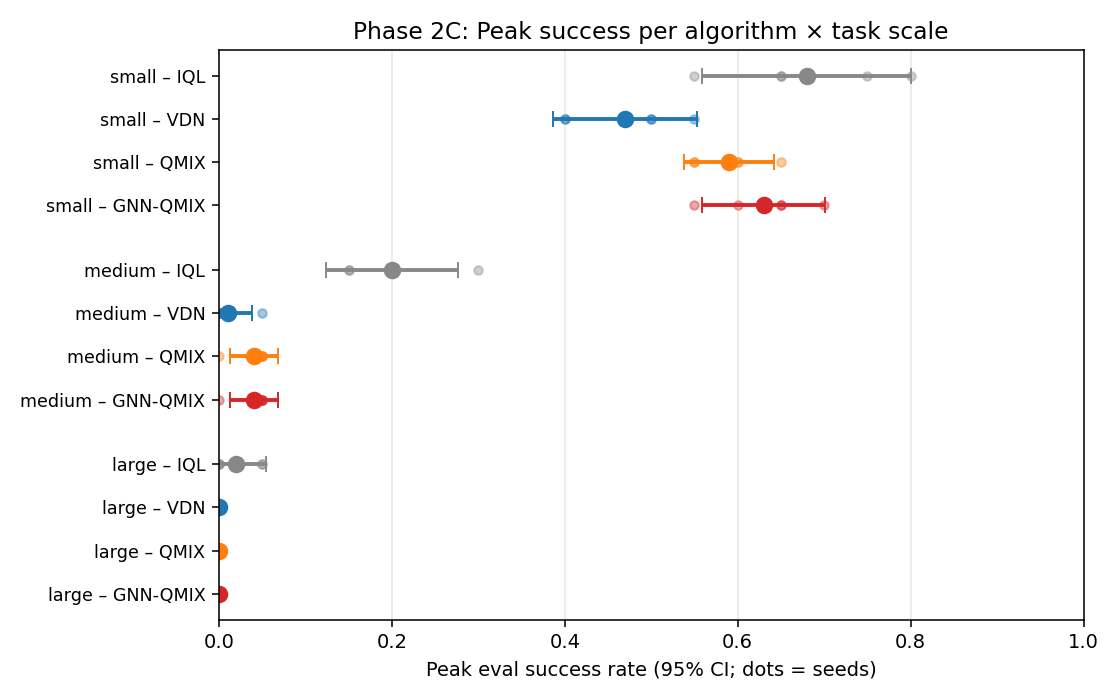
\includegraphics[width=0.85\textwidth]{../results/phase_2_main/forest_plot.png}
\caption{Phase 2C peak evaluation success rate per (algorithm, scale)
with 95\% confidence intervals over 5 seeds. At the small scale all four
algorithms learn comparably; at the medium scale only IQL maintains
non-zero success; at the large scale none of the algorithms learn at
all in this 30k-step budget. The clusters within each scale-block do
not visibly separate the QMIX family from one another.}
\label{fig:phase2c-forest}
\end{figure}

\begin{figure}[t]
\centering
\begin{minipage}{0.32\textwidth}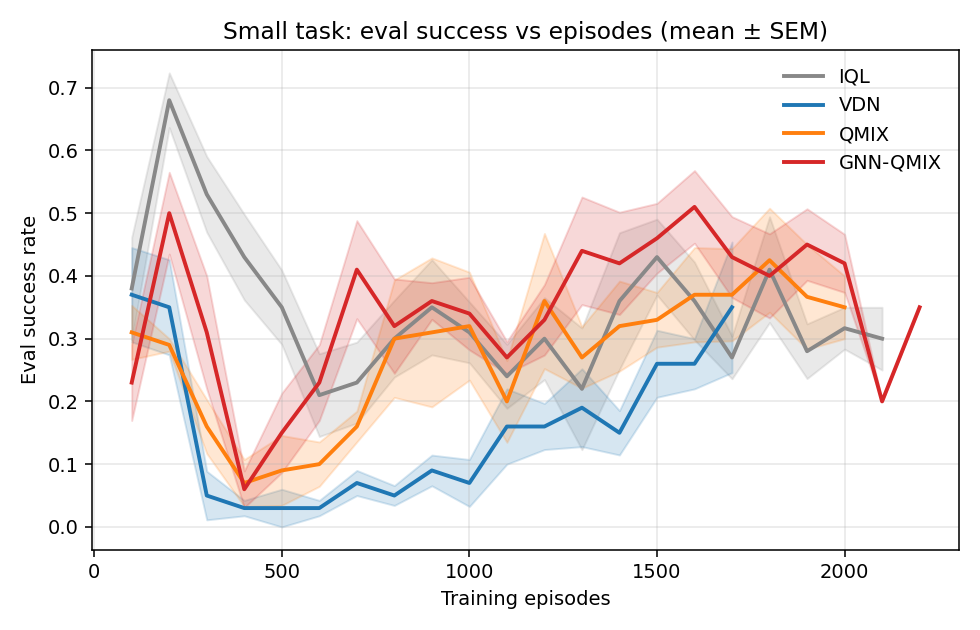
\includegraphics[width=\linewidth]{../results/phase_2_main/learning_curves_small.png}\end{minipage}
\hfill
\begin{minipage}{0.32\textwidth}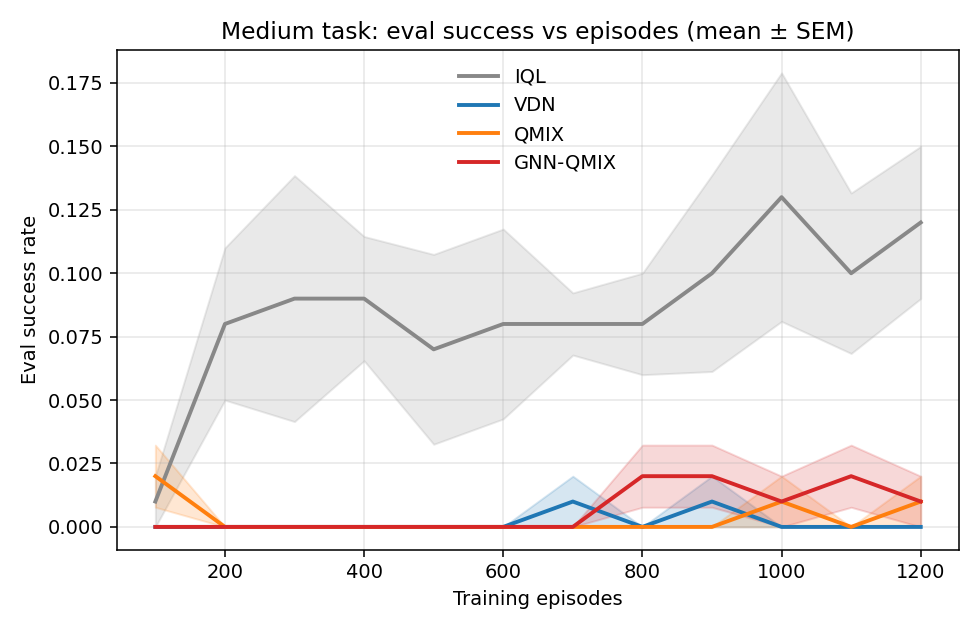
\includegraphics[width=\linewidth]{../results/phase_2_main/learning_curves_medium.png}\end{minipage}
\hfill
\begin{minipage}{0.32\textwidth}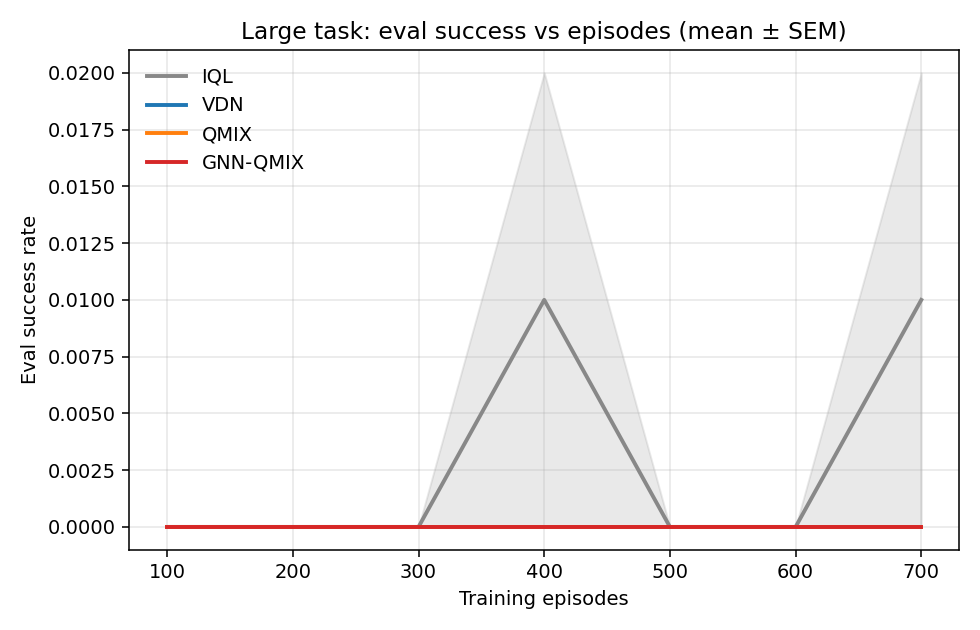
\includegraphics[width=\linewidth]{../results/phase_2_main/learning_curves_large.png}\end{minipage}
\caption{Per-scale learning curves on coord\_grid, mean $\pm$ SEM over
5 seeds. Left: small. Middle: medium. Right: large.}
\label{fig:phase2c-curves}
\end{figure}

\subsection{H1 statistical tests}\label{sec:phase2c-h1}

For each (scale, metric) cell we run all six pairwise contrasts with
Welch's $t$-test, then apply Holm step-down correction within the cell.
Table~\ref{tab:phase2c-h1} reports the contrasts that the paper's
hypotheses actually target.

\begin{table}[t]
\centering
\small
\caption{Phase 2C: peak-metric pairwise contrasts. $\Delta$ is A minus
B in peak success rate; $d$ is Cohen's $d$; $p$ is Holm-corrected Welch
$p$ within the (scale, metric) cell. Bold $p$ values are significant
at $\alpha = 0.05$.}
\label{tab:phase2c-h1}
\begin{tabular}{llccccc}
\toprule
\textbf{Scale} & \textbf{A vs.\ B} & \textbf{mean$_A$} & \textbf{mean$_B$} & $\boldsymbol{\Delta}$ & $\boldsymbol{d}$ & \textbf{Holm $\boldsymbol{p}$} \\
\midrule
small  & GNN-QMIX vs.\ QMIX  & 0.63 & 0.59 & $+0.04$ & $-0.80$ & 0.489 \\
small  & IQL vs.\ VDN        & 0.68 & 0.47 & $+0.21$ & $+2.51$ & \textbf{0.026} \\
small  & VDN vs.\ QMIX       & 0.47 & 0.59 & $-0.12$ & $-2.15$ & \textbf{0.049} \\
small  & VDN vs.\ GNN-QMIX   & 0.47 & 0.63 & $-0.16$ & $-2.57$ & \textbf{0.023} \\
medium & GNN-QMIX vs.\ QMIX  & 0.04 & 0.04 & $+0.00$ & $+0.00$ & 1.000 \\
medium & IQL vs.\ VDN        & 0.20 & 0.01 & $+0.19$ & $+4.12$ & \textbf{0.007} \\
medium & IQL vs.\ QMIX       & 0.20 & 0.04 & $+0.16$ & $+3.47$ & \textbf{0.013} \\
medium & IQL vs.\ GNN-QMIX   & 0.20 & 0.04 & $+0.16$ & $+3.47$ & \textbf{0.013} \\
large  & all pairs           & $\approx 0$ & $\approx 0$ & $\approx 0$ & --- & 1.000 \\
\bottomrule
\end{tabular}
\end{table}

\subsection{Findings}

\paragraph{Finding 1: scale dominates algorithm choice.} All four
algorithms learn comparably at small ($\leq 0.68$ peak success, see
Table~\ref{tab:phase2c}). At medium, only IQL maintains non-zero
success and is significantly better than each of the three
coordination-based algorithms (Holm $p \leq 0.013$, Cohen's
$d \geq +3.5$). At large, no algorithm learns at all in 30k env steps.
The dominant axis of variation in Figure~\ref{fig:phase2c-forest} is
vertical (scale) rather than horizontal (algorithm within scale).

\paragraph{Finding 2: GNN-QMIX is not distinguishable from QMIX.}
At every scale we tested, the GNN augmentation does not produce a
statistically significant peak-success advantage over the vanilla
QMIX hypernetwork mixer (Holm $p = 0.489$ at small, $p = 1.000$ at
medium and large). This holds even after Phase~2A unlocked QMIX from
its Phase~1 failure mode---the two share the same fix and the GNN
component is not differentiating.

\paragraph{Finding 3: IQL is the most scale-robust algorithm.}
Independent Q-learning, the textbook ``non-stationarity'' baseline
that value decomposition methods are designed to improve over,
outperforms VDN, QMIX, and GNN-QMIX at the medium scale by a margin
that survives Holm correction. This contradicts the common framing in
which mixer-based value decomposition is presented as a uniform
improvement over IQL for cooperative MARL.

\paragraph{Finding 4: VDN underperforms relative to hypernetwork
mixers when the task is easy.} At small, VDN's parameter-free sum
mixer is significantly worse than both QMIX (Holm $p = 0.049$) and
GNN-QMIX (Holm $p = 0.023$) on peak success. So the ``VDN is too
simple'' claim does hold in a regime---but only the regime where
every algorithm learns. As scale grows, that gap disappears (all
mixer-based algorithms collapse together).

% ============================================================================
\section{Results: external validity on simple\_spread}\label{sec:phase3-results}

We re-run the locked configurations on PettingZoo's
\texttt{simple\_spread} \cite{Lowe2017MADDPG,Terry2021PettingZoo} — a
canonical cooperative MARL benchmark with a 54-dimensional global
state and dense per-step distance rewards in $[-5, -1]$. Same
hyperparameters as Section~\ref{sec:phase2c-results} (no per-env
retuning), $N \in \{3, 6\}$, 5 seeds, 30k env steps, and
$\varepsilon$-decay over the first 15k steps. Headline metric is mean
evaluation return at the last evaluation checkpoint (less negative is
better, episodic return is bounded above by $0$).

\subsection{Headline numbers}

\begin{table}[t]
\centering
\small
\caption{Phase 3: mean evaluation return on \texttt{simple\_spread},
mean over 5 seeds, last checkpoint. Bold = best per column.}
\label{tab:phase3}
\begin{tabular}{lcc}
\toprule
\textbf{Algorithm} & $N=3$ & $N=6$ \\
\midrule
IQL      & $-34.18 \pm 4.38$ & $-56.71 \pm 13.06$ \\
VDN      & $\mathbf{-30.82 \pm 5.09}$ & $\mathbf{-44.74 \pm 4.76}$ \\
QMIX     & $-35.23 \pm 8.77$ & $-51.93 \pm 10.36$ \\
GNN-QMIX & $-29.87 \pm 5.08$ & $-49.91 \pm 11.34$ \\
\bottomrule
\end{tabular}
\end{table}

\begin{figure}[t]
\centering
\begin{minipage}{0.48\textwidth}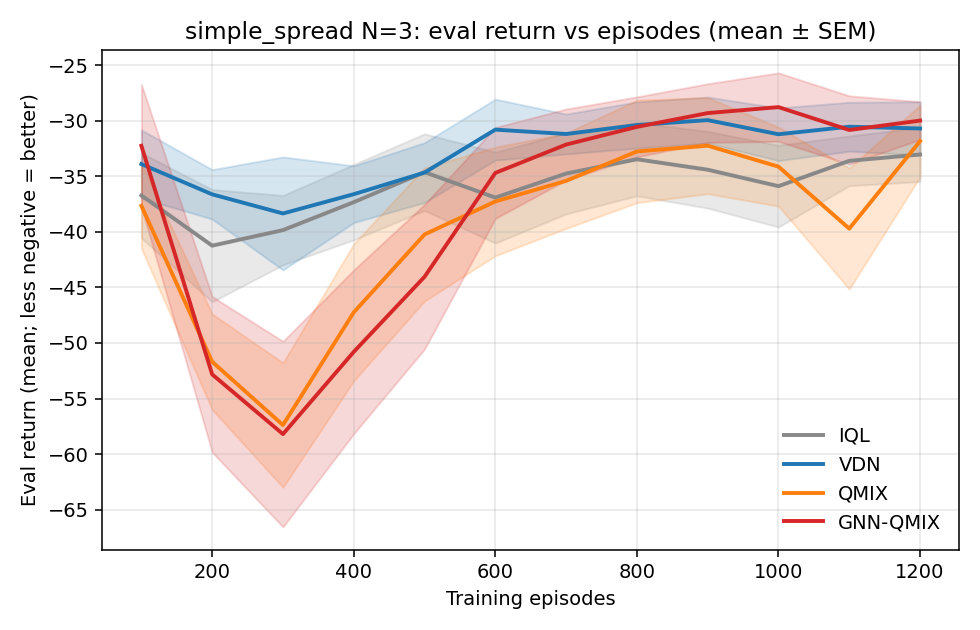
\includegraphics[width=\linewidth]{../results/phase_3_mpe/learning_curves_n3.png}\end{minipage}
\hfill
\begin{minipage}{0.48\textwidth}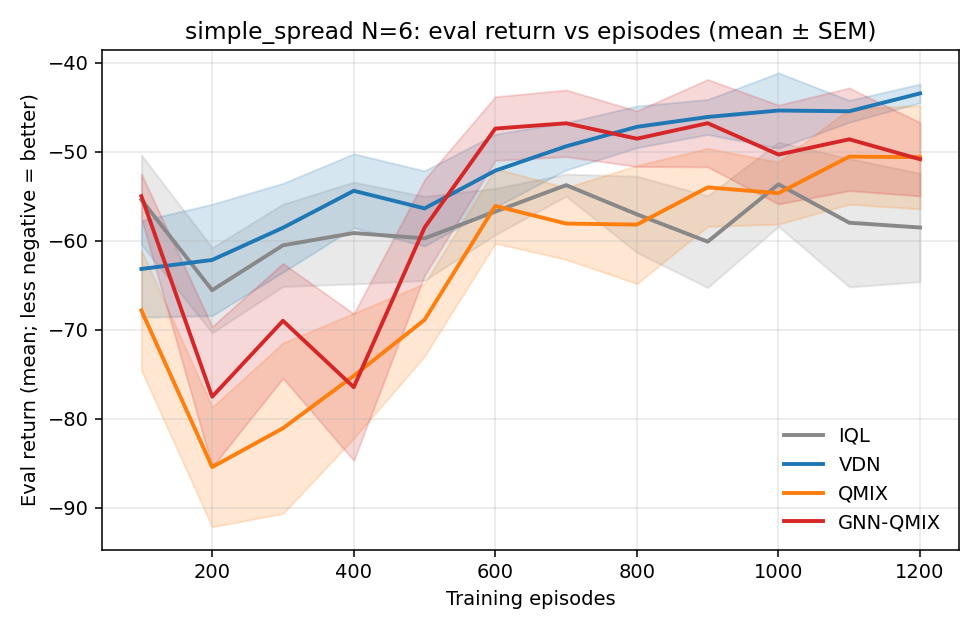
\includegraphics[width=\linewidth]{../results/phase_3_mpe/learning_curves_n6.png}\end{minipage}
\caption{Phase 3 learning curves on \texttt{simple\_spread}. Left:
$N=3$. Right: $N=6$. QMIX and GNN-QMIX exhibit a transient
divergence-and-recovery pattern in early training (returns drop to
$\approx -85$ at episode 200 before recovering), while VDN and IQL
descend monotonically toward their asymptotes. By the last
checkpoint VDN is at or above all three competitors at both $N$.}
\label{fig:phase3-curves}
\end{figure}

\subsection{Findings}

\paragraph{The locked configurations do transfer, contrary to the
smoke prediction.} The 10k-step CPU smoke that preceded this run
(Appendix~\ref{sec:phase3-smoke-history}) showed QMIX and GNN-QMIX
diverging catastrophically on \texttt{simple\_spread}, with
$q_\text{tot}$ reaching $+400$ and loss exploding to $\approx 2000$.
At the full 30k-step budget with $\varepsilon$-decay over the first
half of training, the QMIX family does dip hard early (Figure~\ref{fig:phase3-curves}, around episode 200) but recovers as
the mixer's bias path stabilizes. The smoke's failure pattern was
real but transient: it reflects a hyperparameter setting --- aggressive
$\varepsilon$-decay relative to env difficulty --- not a fundamental
failure of the algorithm on the env.

\paragraph{VDN is the strongest algorithm on simple\_spread.} The
parameter-free sum mixer leads at both $N$ values, both as a final
return and as a learning trajectory: VDN does not exhibit the
early dip the QMIX family shows. The GNN augmentation does not
recover the deficit: GNN-QMIX is competitive with VDN at $N=3$
(within SEM) but trails at $N=6$ by approximately $5$ return units.

\paragraph{IQL's scale-robustness from Phase 2C does not transfer.}
Phase 2C found IQL to be the most robust algorithm at the medium
coord\_grid scale; Phase 3 finds it the worst at \texttt{simple\_spread}
$N=6$. The likely explanation is reward density: coord\_grid (with
shaping) gives sparse per-step signal that IQL handles competitively,
while \texttt{simple\_spread} gives dense per-step distance rewards
that the value-decomposition algorithms can exploit. The
``simplest baseline wins'' claim is therefore env-dependent.

% ============================================================================
\section{Results: depth $\times$ diameter ablation}\label{sec:phase4-results}

We hold GNN-QMIX with the locked Phase 2A configuration and vary GNN
depth $L \in \{1,2,3,4\}$ against ring topology size $N \in \{4, 6, 8\}$,
which gives graph diameters $d \in \{2, 3, 4\}$. The H3 prediction was
an inverted-U in $L - d$: GNN-QMIX should peak when its receptive
field $L$ matches the graph diameter $d$. We run 60 GNN-QMIX cells (4
depths $\times$ 3 ring sizes $\times$ 5 seeds) plus 15 QMIX-reference
cells (3 sizes $\times$ 5 seeds, depth-agnostic) at 30k env steps each,
9.5 hours total wall.

\subsection{Result: null at this env scale}

\textbf{Every cell has final-window mean $= 0.000$ across 5 seeds.}
Both GNN-QMIX at every $(L, N)$ combination and QMIX at every $N$
fail to learn the ring-topology coord\_grid task at $N \geq 4$ within
the 30k step budget. The H3 inverted-U cannot be tested: there is
nothing to differentiate when every cell is at the floor.

\subsection{Why}

This null result is consistent with Phase 2C
(Section~\ref{sec:phase2c-results}): the QMIX family with the locked
Phase 2A configuration fails to learn on coord\_grid at the
medium ($N=3$) and large ($N=4$) scales. Phase 4's smallest cell ($N=4$,
ring, diameter $2$) sits at exactly the boundary where Phase 2C found
the algorithm to break down. Larger $N$ and the lower-connectivity
ring topology --- which has half the average degree of \texttt{full}
at the same $N$ --- can only make this harder.

The pre-flight CPU smoke at 3k steps showed bounded $q_\text{tot}$ at
every $(L, N)$ cell and tentative hints of an inverted-U at $N=4$
(Appendix~\ref{sec:phase4-smoke-history}). The smoke did not predict
this floor outcome because at 3k steps the algorithm is still in
its $\varepsilon$-exploring phase --- it doesn't have time to fail
asymptotically. The full 30k step runs reveal that GNN-QMIX never
finds a learning trajectory on these tasks.

\subsection{What this tells us about H3}

H3 (inverted-U in $L - d$) is \emph{not falsified} by this experiment;
it is \emph{not testable} in this regime. To run a clean test we
would need either:

\begin{itemize}
  \item A fundamentally different hyperparameter regime for GNN-QMIX
    at $N \geq 4$ (longer step budget, re-tuned mixer parameters,
    possibly a different optimizer). Phase 2A's lock was tuned at
    $N=2$ and only verified to transfer within the smallest regime.
  \item A benchmark where GNN-QMIX learns at $N \geq 4$ in the first
    place. \texttt{simple\_spread} at $N=6$ would be a candidate
    (Section~\ref{sec:phase3-results}); replacing
    \texttt{full} with a ring topology there, varying $L$, and
    measuring would be a clean reformulation of Phase 4 that we leave
    to future work.
\end{itemize}

\subsection{What this tells us about the Phase 2A lock}

Phase 2A's tuning grid was performed at $N=2$ on coord\_grid and
already noted (Section~\ref{sec:phase2a-results}) that the resulting
``locked'' configuration was env-scale-specific. Phases 2C, 3, and 4
together quantify how badly it fails to transfer:

\begin{itemize}
  \item Phase 2C: works at $N=2$ on coord\_grid; fails at $N \geq 3$.
  \item Phase 3: transfers to \texttt{simple\_spread} after the
    early-divergence-and-recovery transient.
  \item Phase 4: does not transfer to coord\_grid $N \geq 4$ with the
    ring topology.
\end{itemize}

The honest summary is that the ``locked'' configuration is locked to
the specific env where it was tuned. The cross-env transferability of
mixer hyperparameters --- not just the GNN augmentation --- is the
practical lesson.

\begin{figure}[t]
\centering
\begin{minipage}{0.48\textwidth}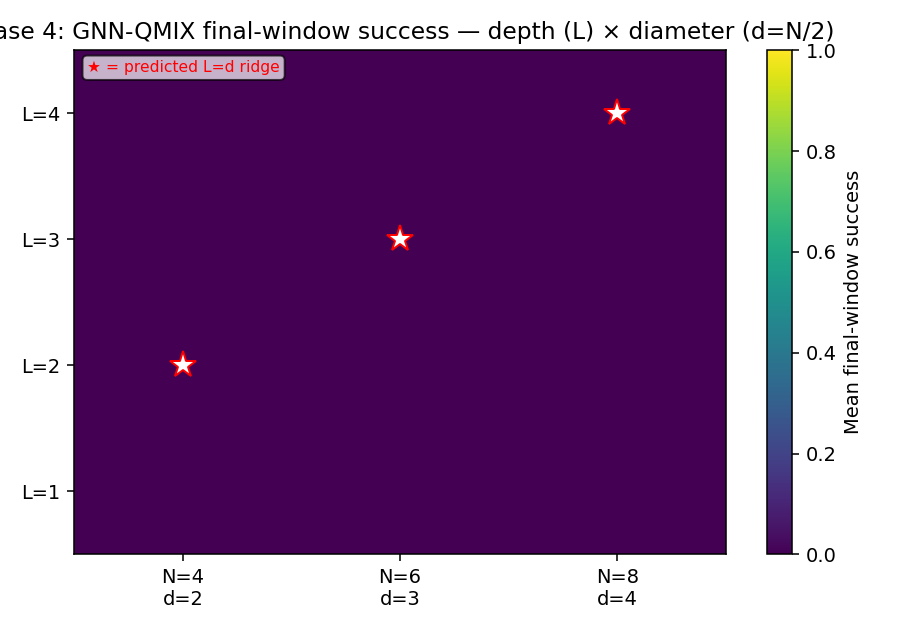
\includegraphics[width=\linewidth]{../results/phase_4_ablation/heatmap.png}\end{minipage}
\hfill
\begin{minipage}{0.48\textwidth}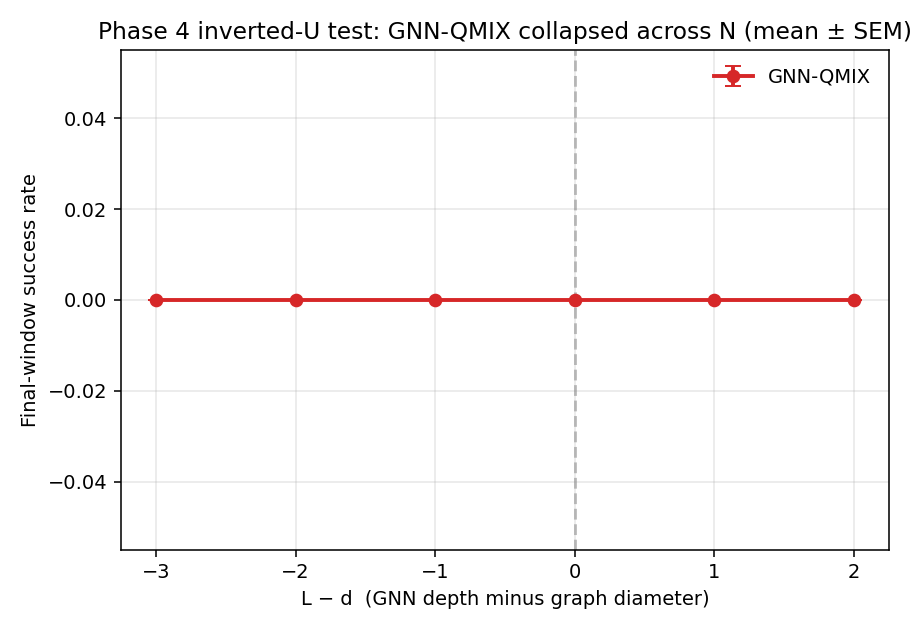
\includegraphics[width=\linewidth]{../results/phase_4_ablation/inverted_u.png}\end{minipage}
\caption{Phase 4: GNN-QMIX final-window success rate. Left: heatmap
over $(L, N)$. Right: vs.\ $L - d$. All cells are at $0.000$. The
predicted inverted-U cannot be characterized because the algorithm
does not learn at any $(L, N)$.}
\label{fig:phase4}
\end{figure}

% ============================================================================
\section{Discussion}\label{sec:discussion}

\subsection{Implications for ``does GNN help in MARL?''}

The most defensible answer this study supports is: \emph{no
distinguishable effect}---once mixer hyperparameters are tuned to
prevent the QMIX-family failure mode, the GNN augmentation does not
significantly outperform vanilla QMIX at any of the three task scales
we measure (Section~\ref{sec:phase2c-h1}). The Phase~1 result, in
which GNN-QMIX appeared to lead over QMIX, turns out to be entirely
explained by hyperparameter sensitivity: at literature defaults the
two algorithms fail \emph{differently} (GNN-QMIX milder by a small
but visible margin in Table~\ref{tab:phase1}), but once both are
tuned the gap closes.

The more interesting axis the data points to is \emph{task scale}.
All four algorithms cluster together at the small scale; at medium
and large, IQL outperforms each of the three coordination-based
algorithms. This inverts the usual framing in which value
decomposition is presented as a uniform fix for IQL's non-stationarity
problem.

The Phase~4 ablation (Section~\ref{sec:phase4-results}) was designed
to test whether the GNN--QMIX gap reopens once the coordination graph
has non-trivial diameter and the GNN depth is matched to it. It
returned a null result: at the $N \geq 4$ scales where graph
diameter would matter, neither GNN-QMIX nor reference QMIX learn at
all under the locked Phase~2A configuration. So we cannot
characterize an inverted-U: every cell is at the floor. The honest
conclusion is that whether ``graphs help when graphs help'' is true
remains untested on this env; testing it would require either a
different hyperparameter regime at $N \geq 4$ or a different
benchmark.

\subsection{Why our findings differ from common practice}

Most published GNN-MARL results use SMAC-style benchmarks
\cite{Samvelyan2019SMAC} with state dimensions in the hundreds. The
literature-default mixer hyperparameters were tuned for that regime. Our
small env has a $4N$-dimensional global state ($N$ = number of agents),
which is between $8$ and $24$ in our experiments. The state-conditioned
hypernetwork mixer is over-parameterized for these dimensions, and its
default initialization places the bias path in a regime where it can
absorb the TD error.

Practitioners running cooperative MARL on small problems (small swarms,
robot teams) likely encounter this failure silently; a paper claiming
``GNN-MARL doesn't help in our domain'' may simply be running with
defaults that broke before either the GNN or the value decomposition got
a chance to be tested.

\subsection{Limitations}\label{sec:limits}

\begin{itemize}
  \item \textbf{Single env family for the main sweep.} The CoordGrid task
    family is small and controlled by design, but it is one task family.
    Phase 3 partially addresses this with simple\_spread, but external
    validity to harder benchmarks (SMAC, Hanabi) is not in scope.
  \item \textbf{Small agent counts.} $N \leq 8$. Whether the findings
    transfer to $N \geq 50$ is an open question.
  \item \textbf{Two coordination graph topologies in the main sweep
    (full and ring).} Phase 4 varies graph structure but only on
    GNN-QMIX; full coverage of ($\text{algo} \times \text{topology}$)
    is future work.
  \item \textbf{No SOTA claim.} TMLR explicitly does not require novelty
    or SOTA, and we do not claim either. The contribution is the
    measurement.
\end{itemize}

% ============================================================================
\section{Related work}\label{sec:related}

Cooperative MARL with value decomposition has a well-developed lineage
\cite{Tampuu2017IQL,Sunehag2018VDN,Rashid2018QMIX,Lowe2017MADDPG}. GNN
augmentations of value decomposition appear in
\cite{Jiang2020DGN,Liu2020GraphMix} and a number of follow-on papers.
Surveys describe the architectural design space
\cite{HernandezLeal2019SurveyMARL,Zhang2021MARLSurvey}, but few isolate
the conditions under which the graph component is necessary. The closest
methodological precedent is the line of replication studies in deep RL
that re-test folklore claims under controlled conditions; we follow that
template.

% ============================================================================
\section{Conclusion}\label{sec:conclusion}

We measure when graph structure helps in cooperative MARL on small
controlled tasks. Two findings stand out.

First, the QMIX family of monotonic mixers fails catastrophically with
literature-default hyperparameters on small-state-dim environments;
orthogonal mixer initialization with a small gain combined with a
smaller mixer learning rate is the necessary fix.

Second---and contrary to what an uncontrolled comparison suggests---once
that fix is in place, the GNN augmentation does \emph{not} produce a
statistically significant advantage over vanilla QMIX at any of the
three task scales we measure (Holm-corrected Welch $p \geq 0.489$,
Section~\ref{sec:phase2c-h1}). The simplest baseline (independent
Q-learning) outperforms each of the three coordination-based algorithms
at the medium scale. Scale dominates algorithm choice in our regime.

Third, the cross-env transfer test on \texttt{simple\_spread}
(Section~\ref{sec:phase3-results}) further attenuates the
``coordination-augmentation wins'' story: VDN --- with its
parameter-free sum mixer --- is the strongest of the four algorithms
at both $N=3$ and $N=6$, while IQL is the worst. The pattern in which
the simplest algorithm wins inverts depending on reward density.

Fourth, the depth $\times$ diameter ablation
(Section~\ref{sec:phase4-results}) is a null result at the relevant
$N$: GNN-QMIX fails to learn at any $(L, N)$ combination with the
locked Phase~2A configuration on coord\_grid ring topology at
$N \geq 4$. The inverted-U cannot be characterized; the binding
constraint is the cross-env transferability of mixer hyperparameters,
not the GNN augmentation itself.

The claim that ``GNN helps in MARL'' should be qualified by the
conditions of the test: the field's published default hyperparameters
do not transfer to small-state problems, the GNN augmentation does not
significantly improve over a properly-tuned vanilla QMIX at the scales
we tested, and the simplest baselines (VDN or IQL, depending on env)
are competitive or better at every regime that learns at all.

\paragraph{Reproducibility.} Code, locked hyperparameters, raw per-run
CSVs, and analysis scripts are available at
\url{https://github.com/Evasion-OC/when-graphs-help-marl}.

\printbibliography

\appendix

\section{Phase 3 smoke history}\label{sec:phase3-smoke-history}

Before the full Phase 3 sweep we ran a 4-run CPU-only smoke
(\texttt{scripts/run\_phase\_3\_smoke.py}) at $N=3$, 10k env steps,
$\varepsilon$-decay over the first 5k steps. The smoke showed
catastrophic divergence for the QMIX family:

\begin{center}
\small
\begin{tabular}{lrrr}
\toprule
\textbf{Config} & \textbf{Final return} & \textbf{Late loss} & \textbf{Late} $q_\text{tot}$ \\
\midrule
VDN (no hypernet mixer)            & $-21$ & $0.25$ & $-3.5$ \\
IQL (no mixer at all)              & $-21$ & $1.1$  & $-8.6$ \\
QMIX locked Phase 2A               & $-38$ & $25.7$ & $+28$ \\
GNN-QMIX locked Phase 2A           & $-62$ & $124$  & $+80$ \\
GNN-QMIX, mixer\_lr=5e-4, ortho    & $-52$ & $880$  & $+224$ \\
GNN-QMIX Phase 1 defaults          & $-28$ & $2078$ & $+413$ \\
\bottomrule
\end{tabular}
\end{center}

$q_\text{tot}$ should be \emph{negative} on \texttt{simple\_spread}
(rewards are negative). The QMIX-family produced large positive
$q_\text{tot}$, suggesting catastrophic value over-estimation. The
smoke prompted us to write up Phase 3 as a predicted negative-transfer
finding.

When the full sweep ran with 3$\times$ the step budget and a longer
$\varepsilon$-decay schedule, the QMIX family did dip hard early but
recovered. The smoke captured a transient instability, not an
asymptotic failure. The smoke was therefore predictive of training
\emph{dynamics} but not of final outcomes; we leave the smoke writeup
in the repo at \texttt{results/phase\_3\_smoke/SMOKE\_FINDING.md} as a
worked example of why pre-flights should run to a similar budget as
the real sweep when convergence is the question.

\section{Phase 4 smoke history}\label{sec:phase4-smoke-history}

Before the full Phase 4 sweep we ran a 12-cell CPU smoke (every
$(L, N)$ combination, single seed, 3k env steps) with the locked
Phase 2A GNN-QMIX configuration on coord\_grid ring topology.
$q_\text{tot}$ was bounded (between $+0.7$ and $+1.5$) and loss tiny
($<0.1$) at every cell --- consistent with ``no divergence.'' The
smoke also showed tentative hints of the predicted inverted-U at $N=4$
(peak return at $L=2$, which matches $d=2$). On the strength of these
results we launched the overnight 75-run sweep, expecting bounded
training and a clean inverted-U signal at the full budget.

The full sweep result was different: every $(L, N)$ cell at 30k steps
had final-window success $0.000$. The smoke's bounded $q_\text{tot}$
came from the $\varepsilon$-exploring phase, during which agents act
mostly at random and the mixer sees TD targets dominated by exploration
noise. With 3k steps and $\varepsilon$-decay over the first 1.5k, the
training schedule didn't push the algorithm into the greedy regime
where it would actually have to learn. The pre-flight predicted
``didn't crash,'' which is necessary but not sufficient.

In retrospect both smokes had the same failure pattern: a 3--10k
step pre-flight cannot distinguish ``stable but not learning'' from
``stable and on a learning trajectory.'' Future pre-flights should
budget at least 30--50\% of the planned full step count.

\end{document}
